% GNUPLOT: LaTeX picture with Postscript
\begingroup
  % Encoding inside the plot.  In the header of your document, this encoding
  % should to defined, e.g., by using
  % \usepackage[cp1252,<other encodings>]{inputenc}
  \inputencoding{cp1252}%
  \makeatletter
  \providecommand\color[2][]{%
    \GenericError{(gnuplot) \space\space\space\@spaces}{%
      Package color not loaded in conjunction with
      terminal option `colourtext'%
    }{See the gnuplot documentation for explanation.%
    }{Either use 'blacktext' in gnuplot or load the package
      color.sty in LaTeX.}%
    \renewcommand\color[2][]{}%
  }%
  \providecommand\includegraphics[2][]{%
    \GenericError{(gnuplot) \space\space\space\@spaces}{%
      Package graphicx or graphics not loaded%
    }{See the gnuplot documentation for explanation.%
    }{The gnuplot epslatex terminal needs graphicx.sty or graphics.sty.}%
    \renewcommand\includegraphics[2][]{}%
  }%
  \providecommand\rotatebox[2]{#2}%
  \@ifundefined{ifGPcolor}{%
    \newif\ifGPcolor
    \GPcolorfalse
  }{}%
  \@ifundefined{ifGPblacktext}{%
    \newif\ifGPblacktext
    \GPblacktexttrue
  }{}%
  % define a \g@addto@macro without @ in the name:
  \let\gplgaddtomacro\g@addto@macro
  % define empty templates for all commands taking text:
  \gdef\gplbacktext{}%
  \gdef\gplfronttext{}%
  \makeatother
  \ifGPblacktext
    % no textcolor at all
    \def\colorrgb#1{}%
    \def\colorgray#1{}%
  \else
    % gray or color?
    \ifGPcolor
      \def\colorrgb#1{\color[rgb]{#1}}%
      \def\colorgray#1{\color[gray]{#1}}%
      \expandafter\def\csname LTw\endcsname{\color{white}}%
      \expandafter\def\csname LTb\endcsname{\color{black}}%
      \expandafter\def\csname LTa\endcsname{\color{black}}%
      \expandafter\def\csname LT0\endcsname{\color[rgb]{1,0,0}}%
      \expandafter\def\csname LT1\endcsname{\color[rgb]{0,1,0}}%
      \expandafter\def\csname LT2\endcsname{\color[rgb]{0,0,1}}%
      \expandafter\def\csname LT3\endcsname{\color[rgb]{1,0,1}}%
      \expandafter\def\csname LT4\endcsname{\color[rgb]{0,1,1}}%
      \expandafter\def\csname LT5\endcsname{\color[rgb]{1,1,0}}%
      \expandafter\def\csname LT6\endcsname{\color[rgb]{0,0,0}}%
      \expandafter\def\csname LT7\endcsname{\color[rgb]{1,0.3,0}}%
      \expandafter\def\csname LT8\endcsname{\color[rgb]{0.5,0.5,0.5}}%
    \else
      % gray
      \def\colorrgb#1{\color{black}}%
      \def\colorgray#1{\color[gray]{#1}}%
      \expandafter\def\csname LTw\endcsname{\color{white}}%
      \expandafter\def\csname LTb\endcsname{\color{black}}%
      \expandafter\def\csname LTa\endcsname{\color{black}}%
      \expandafter\def\csname LT0\endcsname{\color{black}}%
      \expandafter\def\csname LT1\endcsname{\color{black}}%
      \expandafter\def\csname LT2\endcsname{\color{black}}%
      \expandafter\def\csname LT3\endcsname{\color{black}}%
      \expandafter\def\csname LT4\endcsname{\color{black}}%
      \expandafter\def\csname LT5\endcsname{\color{black}}%
      \expandafter\def\csname LT6\endcsname{\color{black}}%
      \expandafter\def\csname LT7\endcsname{\color{black}}%
      \expandafter\def\csname LT8\endcsname{\color{black}}%
    \fi
  \fi
    \setlength{\unitlength}{0.0500bp}%
    \ifx\gptboxheight\undefined%
      \newlength{\gptboxheight}%
      \newlength{\gptboxwidth}%
      \newsavebox{\gptboxtext}%
    \fi%
    \setlength{\fboxrule}{0.5pt}%
    \setlength{\fboxsep}{1pt}%
\begin{picture}(7200.00,5040.00)%
    \gplgaddtomacro\gplbacktext{%
      \csname LTb\endcsname%%
      \put(946,704){\makebox(0,0)[r]{\strut{}$0.02$}}%
      \put(946,1116){\makebox(0,0)[r]{\strut{}$0.03$}}%
      \put(946,1527){\makebox(0,0)[r]{\strut{}$0.04$}}%
      \put(946,1939){\makebox(0,0)[r]{\strut{}$0.05$}}%
      \put(946,2350){\makebox(0,0)[r]{\strut{}$0.06$}}%
      \put(946,2761){\makebox(0,0)[r]{\strut{}$0.07$}}%
      \put(946,3173){\makebox(0,0)[r]{\strut{}$0.08$}}%
      \put(946,3585){\makebox(0,0)[r]{\strut{}$0.09$}}%
      \put(946,3996){\makebox(0,0)[r]{\strut{}$0.1$}}%
      \put(946,4408){\makebox(0,0)[r]{\strut{}$0.11$}}%
      \put(946,4819){\makebox(0,0)[r]{\strut{}$0.12$}}%
      \put(1078,484){\makebox(0,0){\strut{}$30$}}%
      \put(1588,484){\makebox(0,0){\strut{}$32$}}%
      \put(2099,484){\makebox(0,0){\strut{}$34$}}%
      \put(2609,484){\makebox(0,0){\strut{}$36$}}%
      \put(3120,484){\makebox(0,0){\strut{}$38$}}%
      \put(3630,484){\makebox(0,0){\strut{}$40$}}%
      \put(4141,484){\makebox(0,0){\strut{}$42$}}%
      \put(4651,484){\makebox(0,0){\strut{}$44$}}%
      \put(5162,484){\makebox(0,0){\strut{}$46$}}%
      \put(5672,484){\makebox(0,0){\strut{}$48$}}%
      \put(6183,484){\makebox(0,0){\strut{}$50$}}%
      \put(6693,484){\makebox(0,0){\strut{}$52$}}%
    }%
    \gplgaddtomacro\gplfronttext{%
      \csname LTb\endcsname%%
      \put(209,2761){\rotatebox{-270}{\makebox(0,0){\strut{}Intensit\"at [V]}}}%
      \csname LTb\endcsname%%
      \put(6748,2761){\rotatebox{-270}{\makebox(0,0){\strut{}}}}%
      \csname LTb\endcsname%%
      \put(3885,154){\makebox(0,0){\strut{}Motorposition [mm]}}%
      \csname LTb\endcsname%%
      \put(3885,4819){\makebox(0,0){\strut{}}}%
      \csname LTb\endcsname%%
      \put(132,-110){\makebox(0,0)[l]{\strut{}}}%
      \csname LTb\endcsname%%
      \put(5706,4646){\makebox(0,0)[r]{\strut{}Einh\"ullende}}%
      \csname LTb\endcsname%%
      \put(5706,4426){\makebox(0,0)[r]{\strut{}Peaks}}%
    }%
    \gplbacktext
    \put(0,0){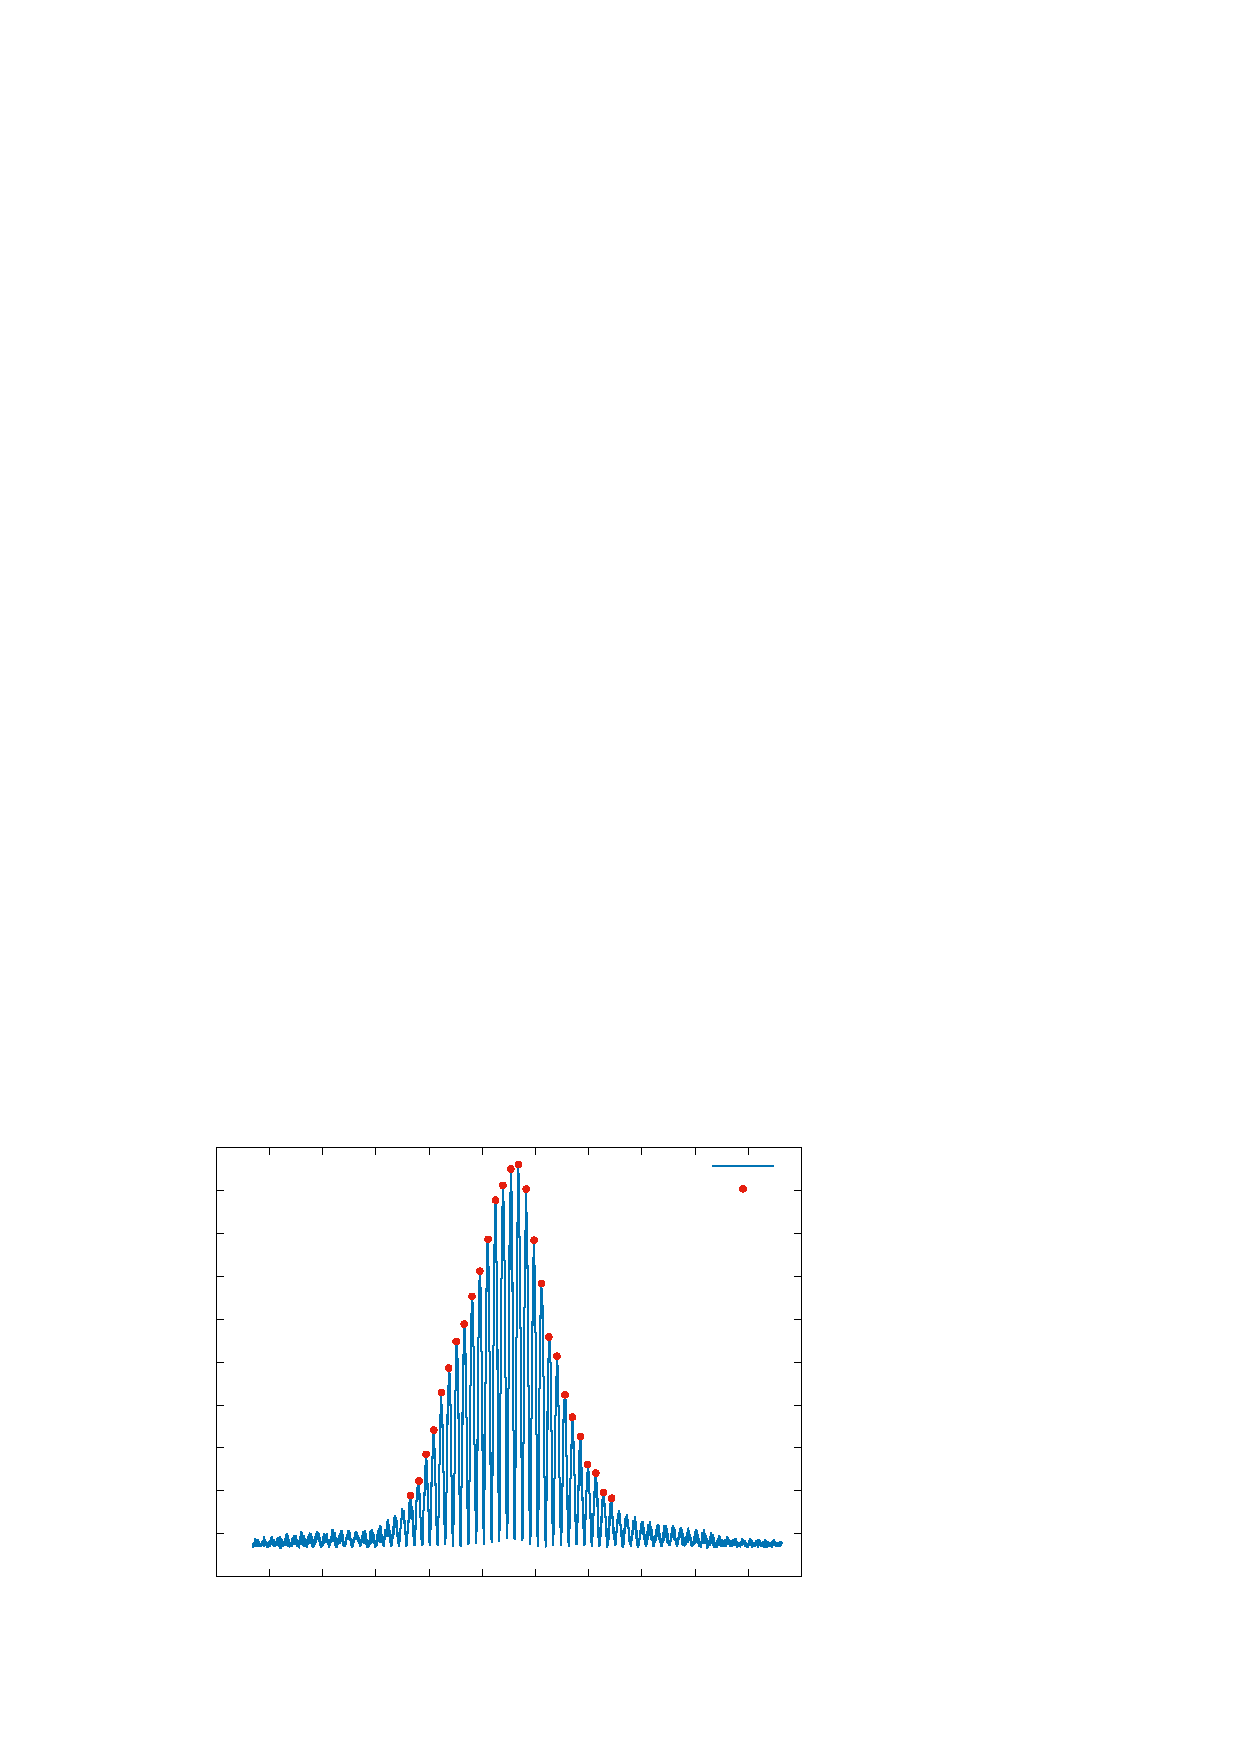
\includegraphics[width={360.00bp},height={252.00bp}]{Dominik/einhuellende_na}}%
    \gplfronttext
  \end{picture}%
\endgroup
